

Portable abstraction of network topologies for high-\/performance computing.

The netloc documentation spans of these sections\+: 
\begin{DoxyItemize}
\item \hyperlink{a00396}{Network Locality (netloc)}, this section below  
\item \hyperlink{a00397}{Netloc with Scotch}  
\end{DoxyItemize}

 \hypertarget{a00396_netloc_summary}{}\section{Netloc Summary}\label{a00396_netloc_summary}
The Portable Network Locality (netloc) software package provides network topology discovery tools, and an abstract representation of those networks topologies for a range of network types and configurations. It is provided as a companion to the Portable Hardware Locality (hwloc) package. These two software packages work together to provide a comprehensive view of the H\+PC system topology, spanning from the processor cores in one server to the cores in another -\/ including the complex network(s) in between.

Towards this end, netloc is divided into two sets of components. The first tools are for the admin to extract the information about the topology of the machines with topology discovery tools for each network type and discovery technique (called readers). The second set of tools is for the user to exploit the collected information\+: to display the topology or create a topology-\/aware mapping of the processes of an application.

 
\begin{DoxyImageNoCaption}
  \mbox{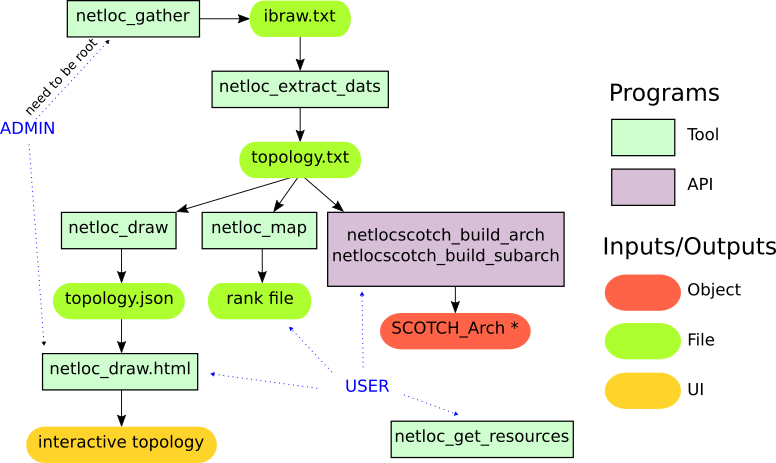
\includegraphics[width=9cm]{netloc_design.png}}
\end{DoxyImageNoCaption}


 \hypertarget{a00396_supportednetworks}{}\subsection{Supported Networks}\label{a00396_supportednetworks}
For now, only Infini\+Band (See \hyperlink{a00396_netloc_setup}{Setup}) is supported, but it is planned to be extended it very soon.

 \hypertarget{a00396_netloc_installation}{}\section{Netloc Installation}\label{a00396_netloc_installation}
The generic installation procedure for both hwloc and netloc is described in \hyperlink{index_common_installation}{Installation}.

Note that netloc is currently not supported on as many platforms as the original hwloc project. netloc is enabled by default when supported, or can be disabled by passing {\ttfamily -\/-\/disable-\/netloc} to the configure command-\/line.

 \hypertarget{a00396_netloc_setup}{}\section{Setup}\label{a00396_netloc_setup}
To use Netloc tools, we need two steps. The first step consists in getting information about network directly from tools distributed by manufacturers. For Infiniband, for instance, this operation needs privileges to access to the network device. For this step we have wrappers in Netloc that will call the right tools with the right options.

The second step will transform the raw files generated by manufacturer tools, into files in a format readable by Netloc tools, and that will not depend on network technologies.

To be clear, let\textquotesingle{}s take an example with Infiniband. This first step is handled by {\ttfamily netloc\+\_\+ib\+\_\+gather\+\_\+raw} that will call {\ttfamily ibnetdiscover} and {\ttfamily ibroutes} tools to generate the necessary raw data files. The step has to be run by an administrator, since the Infiniband tools need to access to the network device.

\begin{DoxyVerb}shell$ netloc_ib_gather_raw --help
Usage: netloc_ib_gather_raw [options] <outdir>
  Dumps topology information to <outdir>/ib-raw/
  Subnets are guessed from the <outdir>/hwloc/ directory where
  the hwloc XML exports of some nodes are stored.
Options:
 --sudo
    Pass sudo to internal ibnetdiscover and ibroute invocations.
    Useful when the entire script cannot run as root.
 --hwloc-dir <dir>
    Use <dir> instead of <outdir>/hwloc/ for hwloc XML exports.
 --force-subnet [<subnet>:]<board>:<port> to force the discovery
    Do not guess subnets from hwloc XML exports.
    Force discovery on local board <board> port <port>
    and optionally force the subnet id <subnet>
    instead of reading it from the first GID.
    Examples: --force-subnet mlx4_0:1
              --force-subnet fe80:0000:0000:0000:mlx4_0:1
 --ibnetdiscover /path/to/ibnetdiscover
 --ibroute /path/to/ibroute
    Specify exact location of programs. Default is /usr/bin/<program>
 --sleep <n>
    Sleep for <n> seconds between invocations of programs probing the network
 --ignore-errors
    Ignore errors from ibnetdiscover and ibroute, assume their outputs are ok
 --force -f
    Always rediscover to overwrite existing files without asking
 --verbose -v
    Add verbose messages
 --dry-run
    Do not actually run programs or modify anything
 --help -h
    Show this help

shell$ ./netloc_ib_gather_raw /home/netloc/data
WARNING: Not running as root.
Using /home/netloc/data/hwloc as hwloc lstopo XML directory.

Exporting local node hwloc XML...
  Running lstopo-no-graphics...

Found 1 subnets in hwloc directory:
 Subnet fe80:0000:0000:0000 is locally accessible from board qib0 port 1.

Looking at fe80:0000:0000:0000 (through local board qib0 port 1)...
 Running ibnetdiscover...
 Getting routes...
  Running ibroute for switch 'QLogic 12800-180 GUID=0x00066a00e8001310 L112' LID 18...
  Running ibroute for switch 'QLogic 12800-180 GUID=0x00066a00e8001310 L108' LID 20...
  Running ibroute for switch 'QLogic 12800-180 GUID=0x00066a00e8001310 L102' LID 23...
  Running ibroute for switch 'QLogic 12800-180 GUID=0x00066a00e8001310 L104' LID 25...
  Running ibroute for switch 'QLogic 12800-180 GUID=0x00066a00e8001310 L106' LID 24...
  Running ibroute for switch 'QLogic 12800-180 GUID=0x00066a00e8001310 L114' LID 22...
  Running ibroute for switch 'QLogic 12800-180 GUID=0x00066a00e8001310 L116' LID 21...
  Running ibroute for switch 'QLogic 12800-180 GUID=0x00066a00e8001310 L109' LID 12...
  Running ibroute for switch 'QLogic 12800-180 GUID=0x00066a00e8001310 L111' LID 11...
  Running ibroute for switch 'QLogic 12800-180 GUID=0x00066a00e8001310 L107' LID 13...
  Running ibroute for switch 'QLogic 12800-180 GUID=0x00066a00e8001310 L103' LID 17...
  Running ibroute for switch 'QLogic 12800-180 GUID=0x00066a00e8001310 L105' LID 16...
  Running ibroute for switch 'QLogic 12800-180 GUID=0x00066a00e8001310 L113' LID 15...
\end{DoxyVerb}


The second step, that can be done by a regular user, is done by the tool {\ttfamily netloc\+\_\+ib\+\_\+extract\+\_\+dats}.

\begin{DoxyVerb}shell$ netloc_ib_extract_dats --help
Usage: netloc_ib_extract_dats <path to input raw data files> <output path> [--hwloc-dir
<hwloc xml path>]
        hwloc-dir can be an absolute path or a relative path from output path

shell$ netloc_ib_extract_dats /home/netloc/data/ib-raw /home/netloc/data/netloc \
  --hwloc-dir ../hwloc
Read subnet: fe80:0000:0000:0000
2 partitions found
        'node'
        'admin'
\end{DoxyVerb}


 \hypertarget{a00396_netloc_draw}{}\section{Topology display}\label{a00396_netloc_draw}
Netloc provides a tool, {\ttfamily netloc\+\_\+draw.\+html}, that displays a topology in a web browser, by using a J\+S\+ON file.\hypertarget{a00396_netloc_draw_setup}{}\subsection{Generate the J\+S\+O\+N file}\label{a00396_netloc_draw_setup}
In order to display a topology, Netloc needs to generate a J\+S\+ON file corresponding to a topology. For this operation, the user must run {\ttfamily netloc\+\_\+draw\+\_\+to\+\_\+json}.

\begin{DoxyVerb}shell$ netloc_draw_to_json --help
Usage: netloc_draw_to_json <path to topology directory>

shell$ netloc_draw_to_json /home/netloc/data/netloc
\end{DoxyVerb}


The {\ttfamily netloc\+\_\+draw\+\_\+to\+\_\+json} command will write a J\+S\+ON file for each topology file found in the input directory. The output files, written also in the input directory, can be open by {\ttfamily netloc\+\_\+draw.\+html} in a web browser.\hypertarget{a00396_netloc_draw_tool}{}\subsection{Using netloc\+\_\+draw}\label{a00396_netloc_draw_tool}
Once the J\+S\+ON file is opened, the rendering is generated by the Javascript vis library for computing the position of the nodes. From the interface, it is possible to search for a specific node, to color the nodes, to expand merged switches, to show statistics, to export as an image... The user can interact with the nodes by moving them. For now, there are bugs and other nodes might move too.

The placement of the nodes is done statically if the topology is detected as a tree. If not, vis.\+js will use physics to find good positions, and it can be very time consuming.

 
\begin{DoxyImageNoCaption}
  \mbox{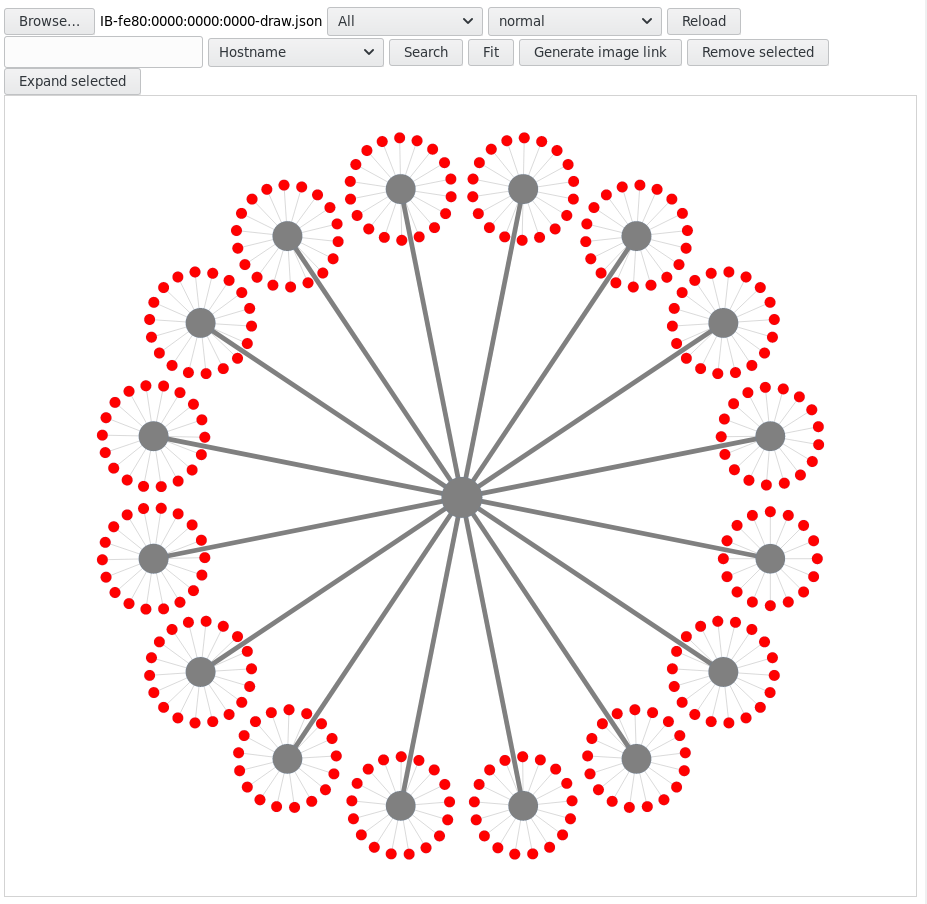
\includegraphics[width=15cm]{netloc_draw.png}}
\end{DoxyImageNoCaption}
 